
\section{Investigation into effects of ODB character (Version-1)}
Before we start need some idea of what sort of P2M to use - real or generated. A real model suffers from the ODB evolution problem (see \ref{XXX}). With a generated P2 model, group activations are spread out over a specified period (say several months) so new groups are appearing in the schedule every day - like the real ODB but in that case they are not entered until required so we dont know about them in advance and cannot take them into account easily.
   
 First set up a few generated P2 models and run some tests - basically use a simple BDS with a fixed environmental scenario and see how some easily calculated and visualized PCM looks - the daily average value of the dynamic contention profile $C_{DC}$ is chosen as it is easily visualized. These tests are all run from 15-oct-07 to 15-dec-07 and have different levels of contention. Table \ref{tab:ltc_p2models} shows details of the phase2 models tested.

\begin{table}[h]
\label{tab:ltc_p2models}
 \begin{center}
  \begin{tabular}{lllll}
   \toprule
   \multicolumn{5}{c}{Phase2 models - more detail required} \\
   \midrule
   DBID & ODB Date & CPlot & NPlot & Description\\
   \midrule
   $P_s$ & 22nov07 midpoint & c1 & p1 & P2Gen small model \\ 
   $P_l$ & 22nov07 midpoint & c3 & p3 & P2Gen light model \\
   $P_m$ & 22nov07 midpoint & c3 & p3 & P2Gen medium model\\
   $P_h$ & 22nov07 midpoint & c2 & p2 & P2Gen heavy model \\
   \midrule
   $O_1$ & 15oct07 snapshot & c4 & p4 & ODB Day 0 Snapshot\\
   $O_2$ & 25sep07 snapshot & c5 & p5 & ODB -20 day snapshot\\
   \bottomrule
  \end{tabular}
 \end{center}
\caption{Phase2 model descriptions - need more info on these than what is in table esp the gen models}
\end{table}

Results for 4 generated models $P_l$ - $P_h$ are shown in figures \ref{fig:c60_gen_av} and \ref{fig:c60_gen_ng}. Similar figures for the ODB snapshots though on a different scale (what does that mean?) are shown in \ref{fig:c60_odb_av} and \ref{fig:c60_odb_ng}.

\begin{figure}[h]
\begin{center}
 \subfigure[Variation of average contention $\bar{C_c}$ for generated phase2 models.] {
   \label{fig:c60_gen_av}
   \includegraphics[scale=0.25, angle=-90]{figures/c60_gen_cav.eps}
  }
 \subfigure[Variation of number of executed groups for generated phase2 models.] {
   \label{fig:c60_gen_ng}
   \includegraphics[scale=0.25, angle=-90]{figures/c60_gen_ng.eps}
  }
 \subfigure[Variation of average contention $\bar{C_c}$ for ODB snapshots.] {
   \label{fig:c60_odb_av}
   \includegraphics[scale=0.25, angle=-90]{figures/c60_odb_cav.eps}
  }
 \subfigure[Variation of number of executed groups for ODB snapshots.] {
   \label{fig:c60_odb_ng}
   \includegraphics[scale=0.25, angle=-90]{figures/c60_odb_ng.eps}
  }
\caption{Comparison of average contention measure and number of groups executed per night for generated phase2 models and ODB snapshots.}
 \end{center}
\end{figure}

From a given generator model (e.g. $P_l$) we can generate any number of actual instances - ideally these would all have the same measurable characteristics (e.g. $\bar{C_c}$) but this is not guaranteed. Tests were run using each of the generator models in order to determine the variation of characteristics. The measurable characteristic chosen was $\bar{C_{dc}}$ - the average dynamic contention over the measurment period. A simple scheduler was chosen using best-score selection and a single $f_{OH}$ metric - i.e. the target which was highest relative to maximum attainable elevation was chosen at each sweep. We are not interested in the scheduler here, only the variability of the generated  P2 characteristics. Simulations were run for the middle 30 days () of the generated models and the values of $\bar{Q_{SU}}$ and $\bar{Q_{XT}}$ are plotted against $\bar{C_c}$ for each model. The results are shown in Fig.~\ref{fig:p2_gen_su} and  Fig.~\ref{fig:p2_gen_xt}.


\begin{figure}[h]
\begin{center}
 \includegraphics[scale=0.5, angle=-90]{figures/p2_gen_qsu.eps}
 \caption[Variation of $Q_{SU}$ with $C_C$ for variable phase2 generator models.] 
   {Variation of $Q_{SU}$ with $C_c$. Each point represents a single phase 2 model generated by one of 4 initial sets of generators.}
\end{center}
\label{fig:p2_gen_su}
\end{figure}


\begin{figure}[h]
 \label{fig:p2_gen_xt}
\begin{center}
 \includegraphics[scale=0.5, angle=-90]{figures/p2_gen_qxt.eps}
 \caption[Variation of $Q_{XT}$ with $C_C$ for variable phase2 generator models.] 
   {Variation of $Q_{XT}$ with $C_c$. Each point represents a single phase 2 model generated by one of 4 initial sets of generators.}
\end{center}
\end{figure}

From the results it is clear there is significant variation in the measurable characteristic for any model though there is a progression between models as might be expected i.e. all the $P_s$ contention values are lower than all the $P_h$ values. There is significant overlap between \emph{adjacent} models. The heavy model generally uses up all or very nearly all of the available night - this is not too surprising - there are more groups to chose from so likely to be few if any slack periods. There is most variation in $Q_{SU}$ for the small models - with low contention there will be periods when no groups are actually schedulable hence the depression of this metric.

